\begin{frame}{Directed acyclic graph}
\label{sec:dag}
% Inference of edges was first tested as a proof-of-concept on a small DAG~(\autoref{fig:dag}). The DAG is designed with 3 protein kinases and 3 transcription factors, with a combination of positive and negative gene regulation control mediated by the TFs, as well as a combination of positive and negative protein activity regulation mediated by the PKs.
\begin{figure}[ht]
    \centering
    \includegraphics[width=0.3\textwidth]{analysis/fig/dag.pdf}
    \caption{\textbf{DAG example.} Pointed/closed arrowhead: edge value = 1, flat/open: -1. }
    \label{fig:dag}
\end{figure}
% As described in~\autoref{sec:equilibrium_model}, each of the six nodes are defined by observations of their simulated log fold-change RNA values as well as defined by their unobserved activity attribute.
Comparing
\begin{itemize}
    \item simple simulation vs. GNW extension
    \item $\boldsymbol{e}$-minimization vs. LLC
\end{itemize}
\end{frame}

\begin{frame}{Directed acyclic graph - simulation}
\begin{columns}
\begin{column}{0.2\textwidth}
Both simulation methods work intuitively
\end{column}
\begin{column}{0.8\textwidth}
\begin{figure}[ht]
\centering
\begin{subfigure}[b]{0.44\textwidth}\centering\caption{}
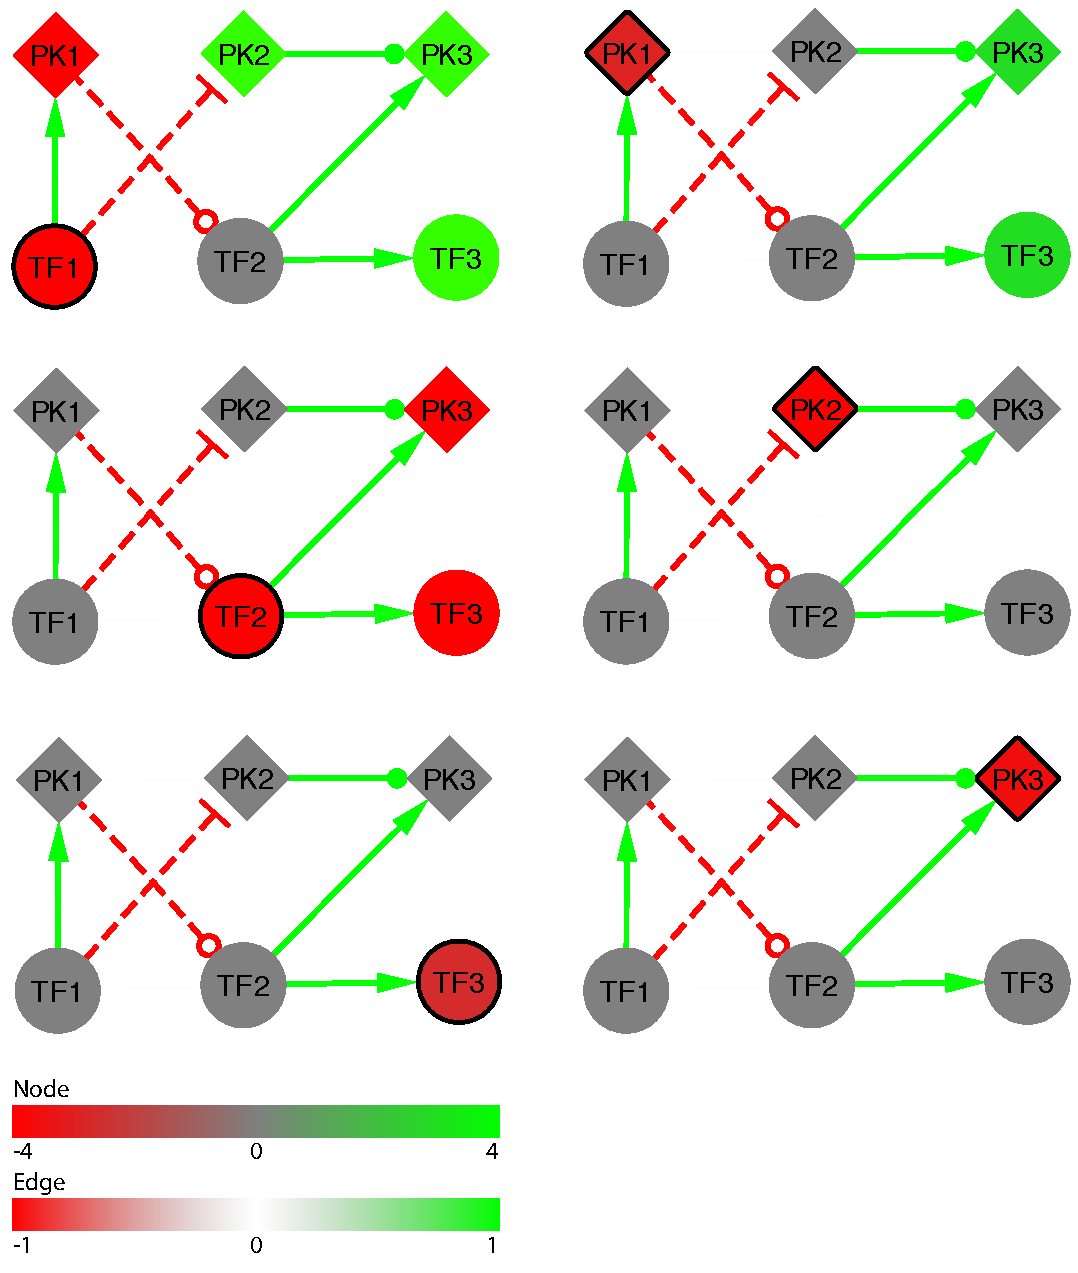
\includegraphics[width=\textwidth]{analysis/fig/prim.pdf}
\end{subfigure}
\hfill
\begin{subfigure}[b]{0.44\textwidth}\centering\caption{}
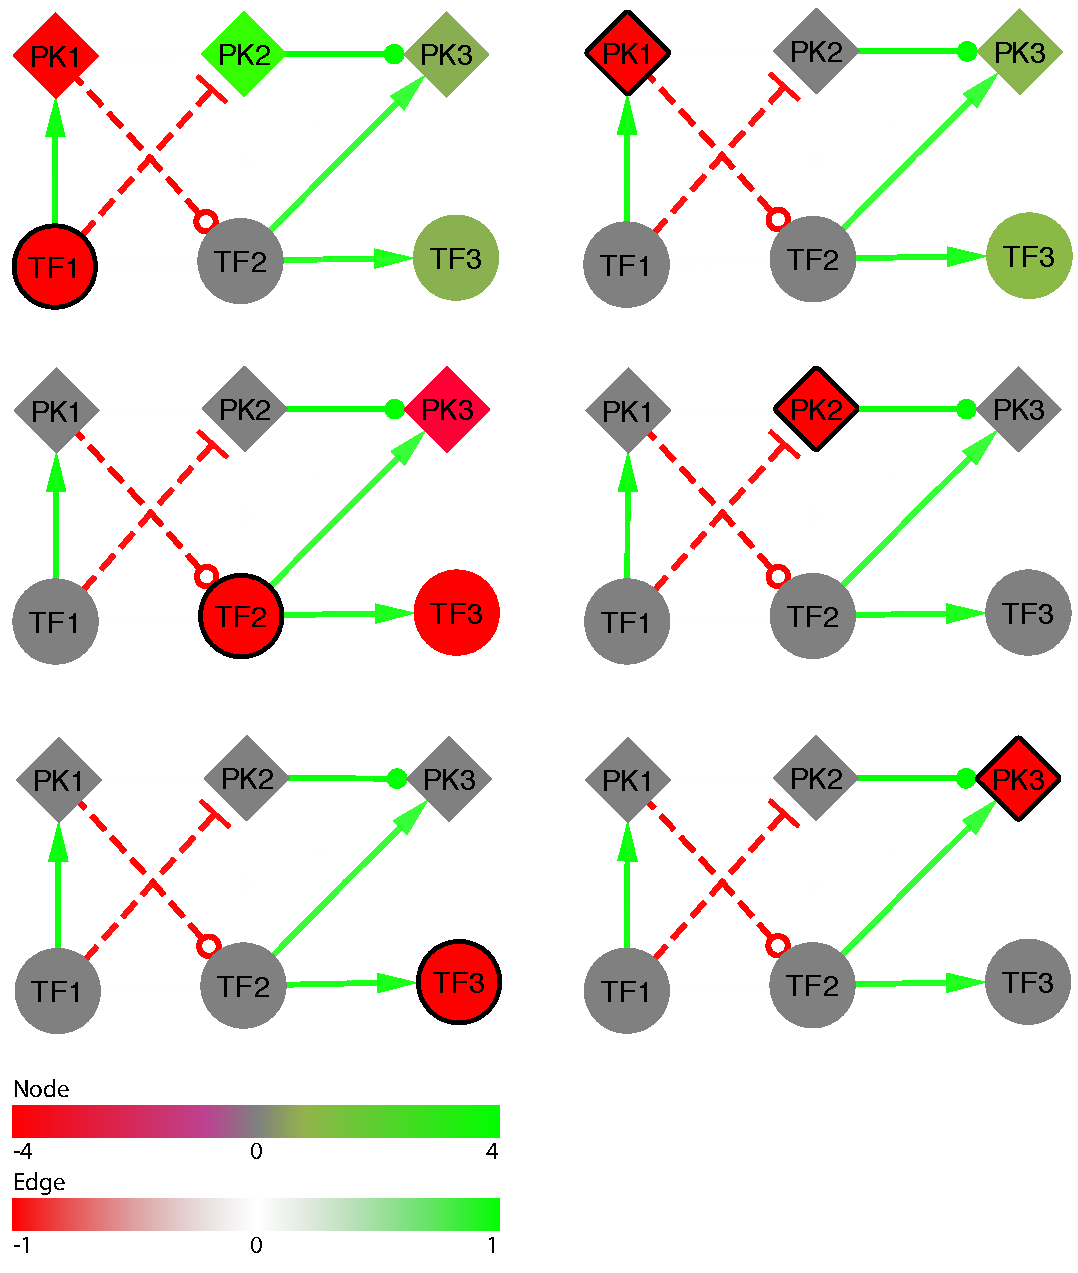
\includegraphics[width=\textwidth]{analysis/fig/gnw.pdf}
\end{subfigure}
\caption{\textbf{DAG node value simulation.} Simple iterative simulation~(a), and extended GeneNetWeaver~(b). LogFC node values. \textcolor{black}{black border} = gene deletion. Edges: true graph. }
\label{fig:dag_data}
\end{figure}

% Two different methods of node value simulation was applied, with the resulting node values indicating with node coloring in~\autoref{fig:dag_data}, where the edges are simply showing the true graph from~\autoref{fig:dag}. The first method is using the inference equations in the simple iterative simulation described in~\autoref{sec:prim}. The second method is applying the GeneNetWeaver kinase extension~(\autoref{sec:gnw_extension}), which is the more realistic simulation approach applying nonlinear gene regulation mechanisms.



% We see how PK regulatory interactions are not directly observed but still detectable through a regulated transcription factor. We also see that the node values are less pronounced when simulated using the GNW extension but otherwise identical in this simple example. Both methods are displaying node values that intuitively would be expected for each given knockout.
\end{column}
\end{columns}
\end{frame}

\begin{frame}{Directed acyclic graph - Inference}

% The $\boldsymbol{e}$-minimization method of edge inference is compared to the original edge inference method LLC~(\autoref{sec:eberhardt}) by using each for edge inference on the simulated node values. The inferred edges on node values simulated using either the simple method or GNW extension are shown in~\autoref{fig:dag_infer}.


\begin{figure}[ht]
\centering
\begin{subfigure}[b]{0.23\textwidth}\centering\caption{}
\includegraphics[width=\textwidth]{analysis/fig/weight.pdf}\label{fig:dag_infer.a}
\end{subfigure}
\hfill
\begin{subfigure}[b]{0.23\textwidth}\centering\caption{}
\includegraphics[width=\textwidth]{analysis/fig/gnwweight.pdf}
\end{subfigure}
\hfill
\begin{subfigure}[b]{0.23\textwidth}\centering\caption{}
\includegraphics[width=\textwidth]{analysis/fig/B.pdf}\label{fig:dag_infer.c}
\end{subfigure}
\hfill
\begin{subfigure}[b]{0.23\textwidth}\centering\caption{}
\includegraphics[width=\textwidth]{analysis/fig/gnwB.pdf}
\end{subfigure}
\vskip\baselineskip
\begin{subfigure}[b]{0.25\textwidth}\centering
\includegraphics[width=\textwidth]{analysis/fig/edge_legend.pdf}
\end{subfigure}
\caption{\textbf{DAG edge inference.}  $\boldsymbol{e}$-minimization~(a,b), and LLC~(c,d). On simple iterative simulation~(a,c), and GeneNetWeaver kinase extension~(b,d).}
\label{fig:dag_infer}
\end{figure}
$\boldsymbol{e}$-minimization captures indirectness, LLC does not
% We see that LLC correctly predicts the TF edges, which are directly influencing node values, but does not capture any edges from the protein kinases, which are indirectly affecting node values~\autoref{fig:dag_infer.c}. We further see that the $\boldsymbol{e}$-minimization method captures all detectable edges~\autoref{fig:dag_infer.a}. The PK edge from $\text{PK}_2$ to $\text{PK}_3$ is undetectable since $\text{PK}_3$ does not regulate anything. For node values simulated with GNW extension it is the same observations, although some edges appear weaker, which can make them harder to detect in noisy data. However, since edge inference is a boolean classification problem, their weakness is not an issue as long as the edge value is above the threshold used for edge detection.


\end{frame}
